\documentclass[tikz, border=4pt]{standalone}
\usepackage{tikz}
\usetikzlibrary{arrows.meta}
\begin{document}
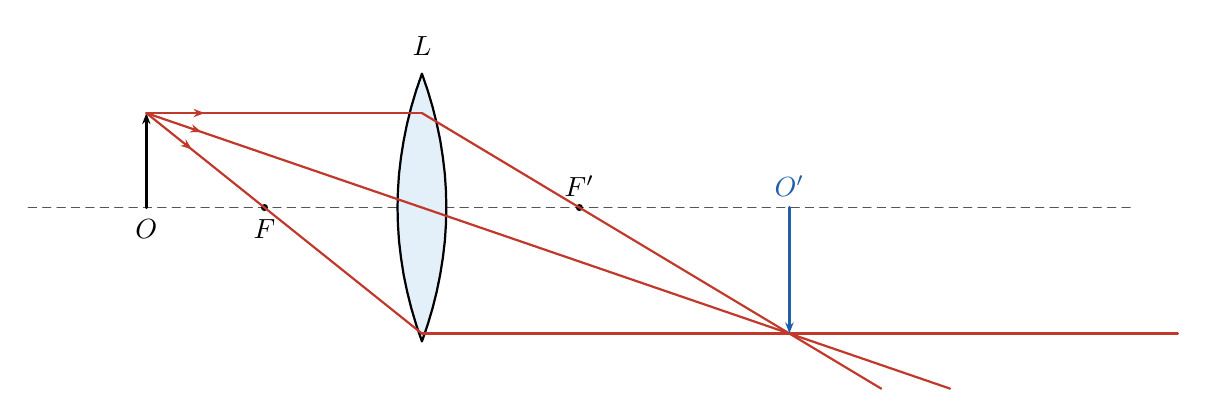
\begin{tikzpicture}[x=1cm, y=1cm]
  \definecolor{tdc1}{HTML}{555555}
  \definecolor{tdc2}{HTML}{E3F0FA}
  \definecolor{tdc3}{HTML}{C0392B}
  \definecolor{tdc4}{HTML}{1F5FA8}

  % physics: Optics (DiagramTeX)
  \begin{scope}[shift={(5.06,-2.32)}, line cap=round, line join=round]
  \draw[tdc1, line width=0.4pt, dash pattern=on 3pt off 2.2pt] (-5,0) -- (9,0);
  \filldraw[fill=tdc2, draw=black, line width=0.8pt] (0,-1.7) -- (0.073,-1.488) -- (0.136,-1.275) -- (0.189,-1.063) -- (0.232,-0.85) -- (0.266,-0.637) -- (0.291,-0.425) -- (0.305,-0.213) -- (0.31,0) -- (0.305,0.212) -- (0.291,0.425) -- (0.266,0.637) -- (0.233,0.85) -- (0.189,1.063) -- (0.136,1.275) -- (0.073,1.488) -- (0,1.7) -- (0,1.7) -- (-0.073,1.488) -- (-0.136,1.275) -- (-0.189,1.063) -- (-0.232,0.85) -- (-0.266,0.637) -- (-0.291,0.425) -- (-0.305,0.213) -- (-0.31,0) -- (-0.305,-0.212) -- (-0.291,-0.425) -- (-0.266,-0.637) -- (-0.233,-0.85) -- (-0.189,-1.063) -- (-0.136,-1.275) -- (-0.073,-1.488) -- (0,-1.7) -- cycle;
  \node at (0,2.047) {$L$};
  \fill (-2,0) circle (1.28pt);
  \node at (-2,-0.272) {$F$};
  \fill (2,0) circle (1.28pt);
  \node at (2,0.272) {$F'$};
  \draw[line width=1.2pt, -{Stealth[length=4pt]}] (-3.5,0) -- (-3.5,1.2);
  \node at (-3.5,-0.273) {$O$};
  \draw[tdc3, line width=0.8pt] (-3.5,1.2) -- (0,1.2);
  \draw[tdc3, line width=0.8pt, -{Stealth[length=4pt]}] (-2.84,1.2) -- (-2.76,1.2);
  \draw[tdc3, line width=0.8pt] (0,1.2) -- (5.833,-2.3);
  \draw[tdc3, line width=0.8pt] (-3.5,1.2) -- (0,0);
  \draw[tdc3, line width=0.8pt, -{Stealth[length=4pt]}] (-2.876,0.986) -- (-2.8,0.96);
  \draw[tdc3, line width=0.8pt] (0,0) -- (6.708,-2.3);
  \draw[tdc3, line width=0.8pt] (-3.5,1.2) -- (0,-1.6);
  \draw[tdc3, line width=0.8pt, -{Stealth[length=4pt]}] (-2.985,0.788) -- (-2.922,0.738);
  \draw[tdc3, line width=0.8pt] (0,-1.6) -- (9.6,-1.6);
  \draw[tdc4, line width=1.2pt, -{Stealth[length=4pt]}] (4.667,0) -- (4.667,-1.6);
  \node[text=tdc4] at (4.667,0.273) {$O'$};
  \end{scope}
\end{tikzpicture}
\end{document}
